\section{GPaaScaler architecture}

This section presents our auto-scaler architecture named \emph{GPaaScaler}, which continuously listens the instances of events \emph{e.g.,} response time, green energy availability, working modes of application etc., pushed by SaaS(Software-as-a-Service) and IaaS(Infrastructure-as-a-Service) layers in a changing environment. Furthermore, it inherits the capability to actuate both at application and at infrastructure level.
We use the most popular self-adaptive design framework: Monitor-Analyze-Plan-
Execute-Knowledge (MAPE-K) loop \cite{vision} for our auto-scaler.
Our contribution lies on the \emph{analyze} and \emph{plan} (A-P) block of this autonomic framework.


\begin{figure} [ht]
\centering
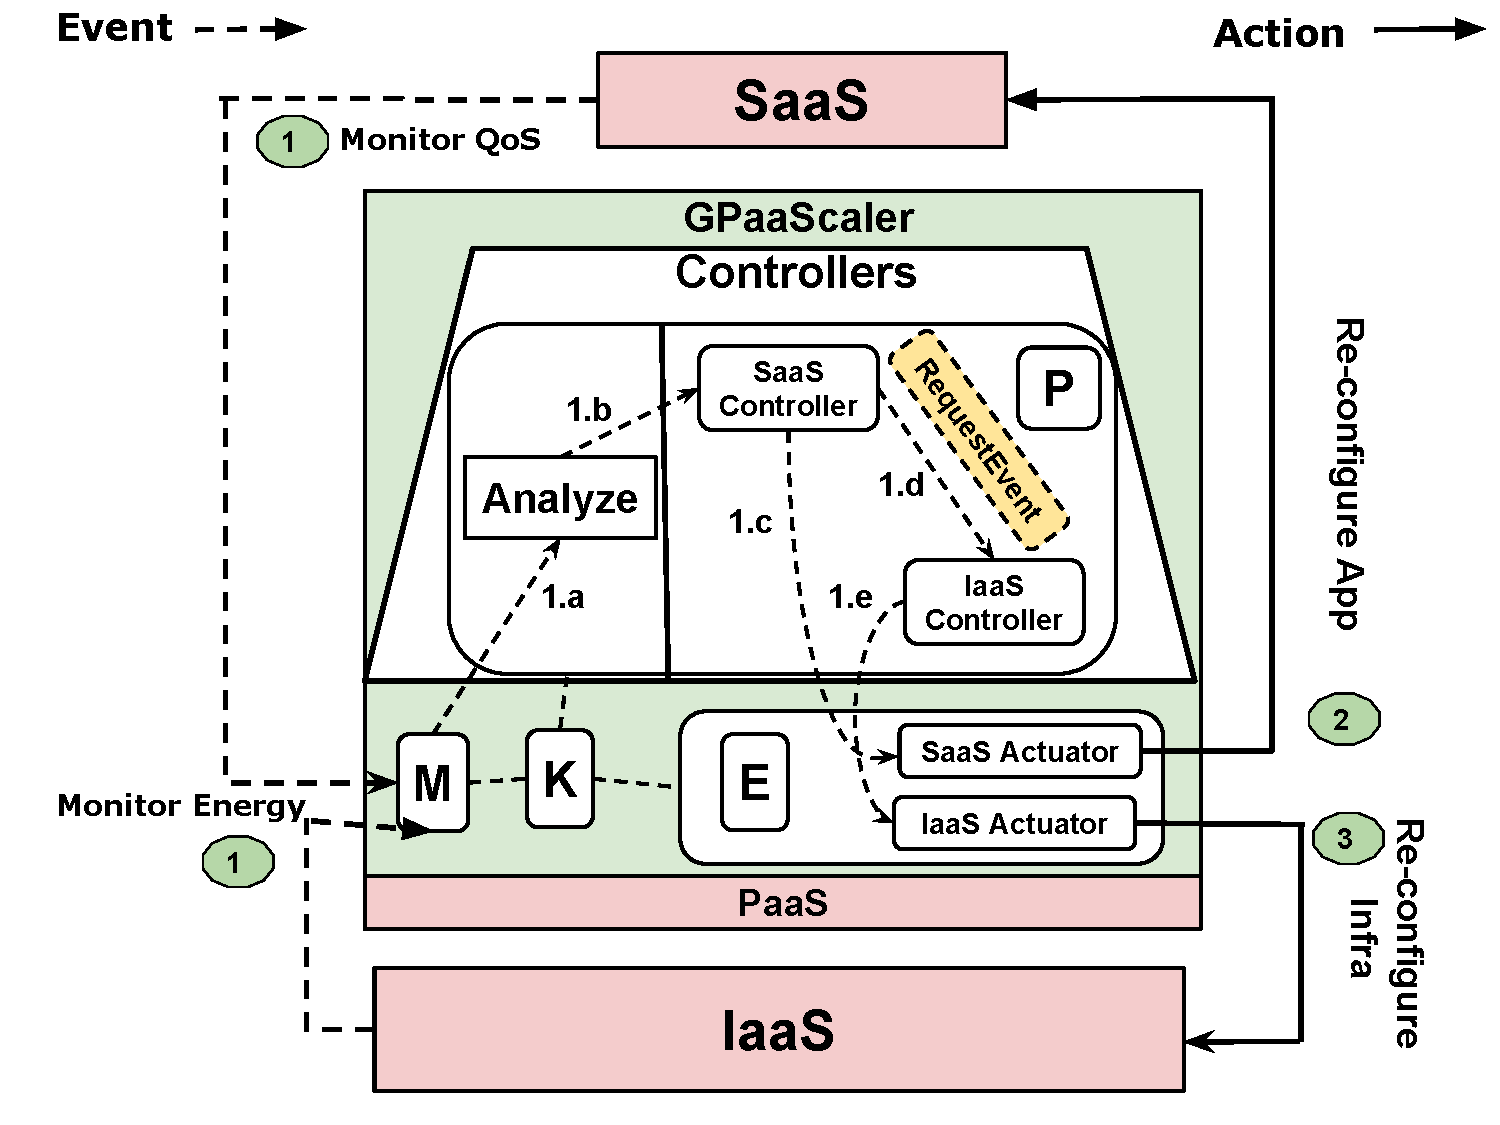
\includegraphics[scale=.35]{Graphs/test_gpaascaler.pdf}
\caption{GPaaScaler architecture}
\label{fig:GPaaScaler}
\end{figure}

Figure \ref{fig:GPaaScaler} presents the sequential control flow of the event in an ordered way (from $1.a$ to $1.e$). 
Monitoring (M) block pushes listened events to \emph{Analyze} block via ($1.a$) from SaaS layer (\emph{i.e.,} response time, workload, application's working mode, etc.) and from IaaS layer (\emph{i.e.,} quality of energy). Analyze (A) block is responsible for analyzing and decoupling events to extract the pertinent information and feed appropriate event to the event handler at the SaaS controller via $1.b$ flow. Once the events are 
received, Plan (P) block analyzes and matches to the predefined reactive or proactive rules and creates a
configuration plan. The block pushes information through $1.c$ and $1.e$ to
Execution (E) block, which consists of two types of actuator \emph{i.e.,} SaaS and IaaS. These actuators act as an API to execute the action at application and at infrastructure layer respectively.
Therefore, After the configuration plan, if needed, SaaS controller triggers action through SaaS actuator.

Most of the popular cloud applications provides some extra features (\emph{e.g.,} several product recommendation in an e-commerce application), which enhances user’s quality of experience (QoE), but is not the core functionality of the service. These independent application
components can be isolated to be activated/deactivated to provide different service levels to the end users. Different service levels can be also adopted to other Cloud applications, such as: (i) 2D/3D interactive applications over network (\emph{e.g.,} architectural features where the rendering could be customized); (ii) On-line itineraries on maps with different details (\emph{e.g.,} points of interest), etc.
For the sake of generality, we propose three user experience levels. Mode High refers to high user
experience while Mode Medium and Mode Low indicate to medium and low user experience respectively (see Figure \ref{fig:modes}). 
When current application behavior deviates from target system state in terms of SLA, the auto-scaler gracefully downgrades the user experience from higher mode to lower mode and vice-versa through proper actuator value. Once SaaS actuator triggers the adaptation plan, it passes request for addition/removal of resources event as «RequestEvent» to IaaS controller if the former controller decides that application needs more/less resources, which is shown at Figure \ref{fig:GPaaScaler}. Following the event, IaaS controller decides to take action via traditional infrastructure API (built in IaaS actuator) that is \emph{scale-in} and \emph{scale-out} or wait/discard the request issued by the SaaS controller.
In addition, \encircle{1}, \encircle{2} and \encircle{3} depict the task flow of our auto-scaler.
In summary, IaaS controller only gets activated if SaaS controller issues any «RequestEvent». Since the public IaaS provider's does not expose their resource allocation policies to the upper layers \emph{i.e.,} PaaS or SaaS, we consider infrastructure as a black box. Therefore, our proposed IaaS controller are unaware of resource allocation strategy, for instance, what types of VM is to be added/removed or location of VM's in specific servers etc.




\begin{figure} [ht]
\centering
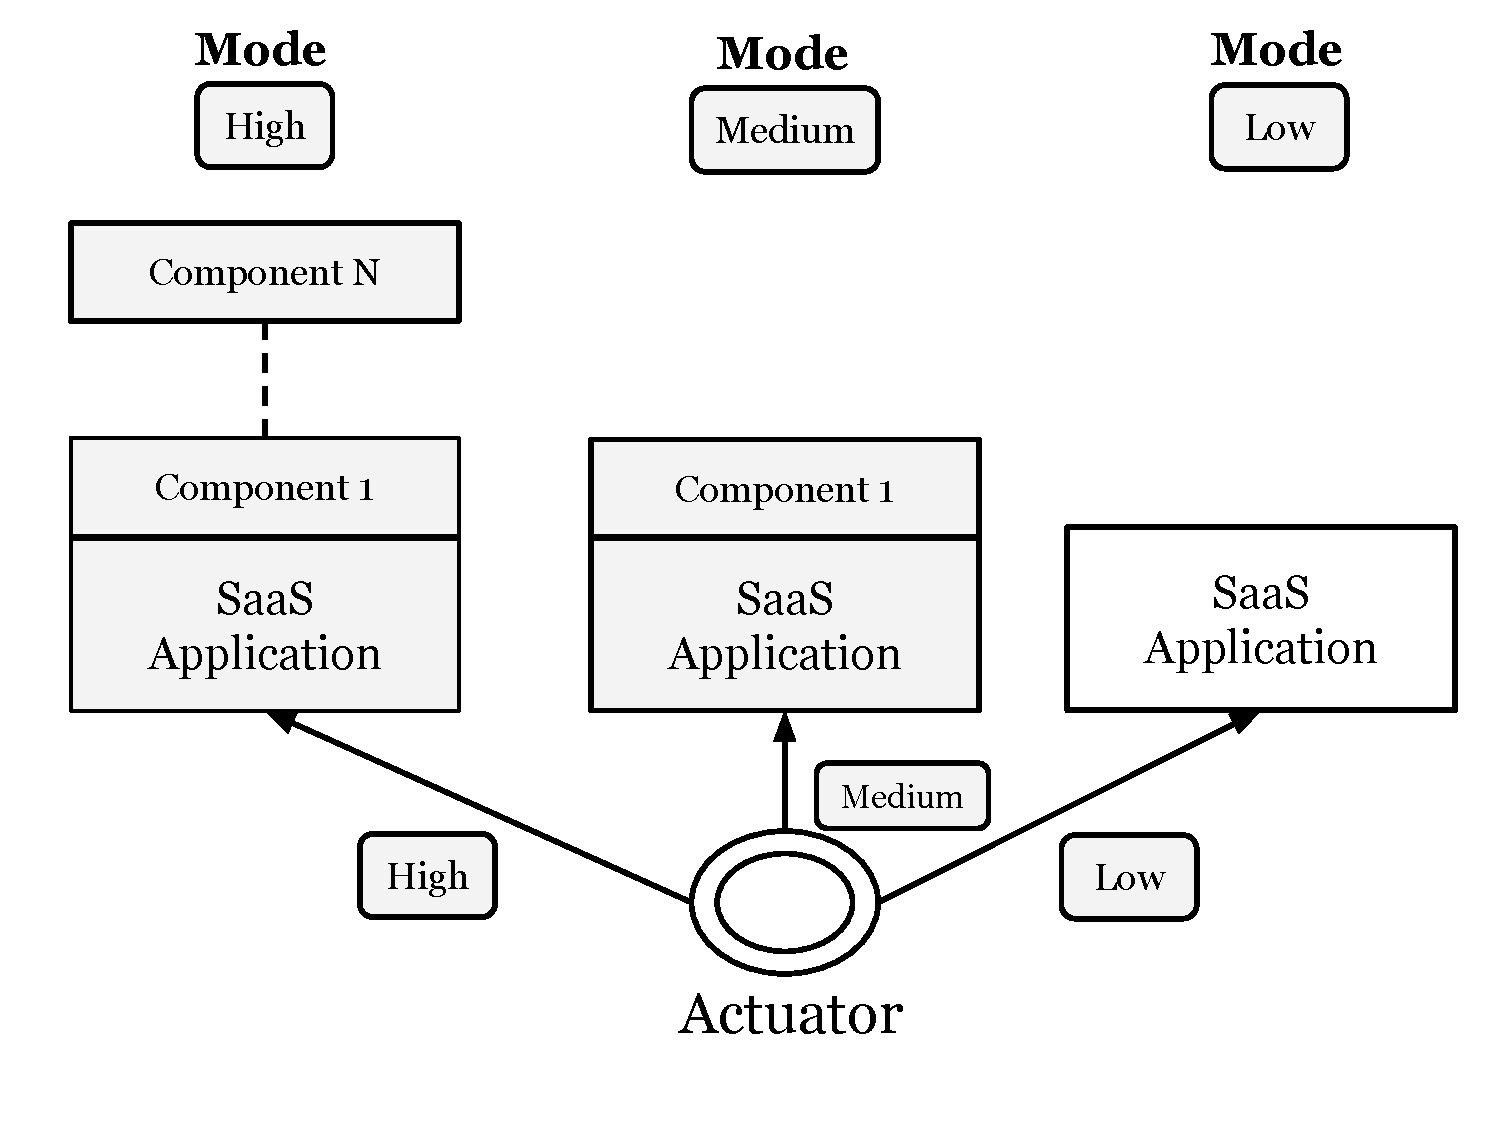
\includegraphics[scale=.32]{Graphs/action_1.pdf}
\caption{Applications mode under different service level}
\label{fig:modes}
\end{figure}

%«RequestEvent»